\documentclass[12pt, a4paper]{article}

% --- Codificação e língua ---
\usepackage[utf8]{inputenc}
\usepackage[T1]{fontenc}
\usepackage[brazil]{babel}

% --- Matemática ---
\usepackage{amsmath}
\usepackage{amssymb}

% --- Tabelas e figuras ---
\usepackage{booktabs}
\usepackage{graphicx}
\usepackage{float}
\usepackage{caption}
\usepackage{subcaption}
\usepackage{adjustbox}
\usepackage{array}
\usepackage{multirow}
\usepackage{xcolor}
\usepackage{tcolorbox}
\usepackage{enumitem}

% --- Caminho das figuras ---
% Este .tex deve estar em forecasting_inflation/results/
% As imagens devem estar na mesma pasta (baixe com o script setup_figs.sh)
\graphicspath{{./}}

% --- Margens ---
\usepackage[top=2.5cm, bottom=2cm, left=2.5cm, right=2cm]{geometry}

% --- Espaçamento ---
\usepackage{setspace}
\onehalfspacing

% --- Hiperlinks ---
\usepackage[colorlinks=true, linkcolor=teal,
            citecolor=teal, urlcolor=teal]{hyperref}

% --- Caixas de destaque ---
\tcbuselibrary{skins, breakable}
\newtcolorbox{destaque}[1][]{
  colback=teal!5!white, colframe=teal!60!black,
  fonttitle=\bfseries, title=#1,
  breakable, before skip=10pt, after skip=10pt
}
\newtcolorbox{atencao}[1][]{
  colback=orange!5!white, colframe=orange!70!black,
  fonttitle=\bfseries, title=#1,
  breakable, before skip=10pt, after skip=10pt
}

% ============================================================
\begin{document}

% --- Capa simples ---
\begin{titlepage}
  \centering
  \vspace*{2cm}
  {\Large \textbf{Previsão de Inflação com Parâmetros Variando no Tempo}\par}
  \vspace{0.5cm}
  {\large Modelo 2SRR aplicado ao CPIAUCSL (FRED-MD)\par}
  \vspace{1.5cm}
  {\normalsize
    \textbf{Hiperparâmetros da especificação principal:}\\[0.3em]
    $K_{\max} = 40$ componentes PCA \quad|\quad
    Variância explicada $\geq 90\%$ \quad|\quad
    $k$\text{-fold} $= 5$\\[0.3em]
    312 janelas fora da amostra \quad|\quad
    Janeiro de 1960 a junho de 2025
  }
  \vspace{1.5cm}
  {\large Felipe Dornelles\par}
  \vspace{0.5cm}
  {\normalsize TCC --- UFRGS\par}
  \vspace{0.5cm}
  {\normalsize \today\par}
  \vfill
  \begin{atencao}[Nota sobre este documento]
    Este é um relatório intermediário de resultados, produzido
    com assistência de IA para resumir os resultados com o
    objetivo de apresentar e discutir os outputs gerados até o momento.
    \textbf{Não é o trabalho final.} Serve para alinhar o entendimento
    dos resultados com o orientador antes da redação definitiva.
  \end{atencao}
\end{titlepage}

\tableofcontents
\newpage

% ============================================================
\section{O que foi feito e por quê}
\label{sec:contexto}

Este trabalho aplica o modelo \textbf{2SRR} (\textit{Two-Step
Ridge Regression} com parâmetros variantes no tempo), proposto
por \textbf{Coulombe (2024)}, ao problema de previsão da inflação
americana medida pelo CPIAUCSL.

A ideia central é simples: e se os coeficientes de uma regressão
não fossem fixos, mas pudessem \emph{mudar ao longo do tempo},
acompanhando as transformações da economia? Coulombe demonstra
que essa formulação é algebricamente equivalente a um modelo
Ridge em que a penalidade recai sobre as \emph{mudanças} dos
coeficientes entre períodos --- não sobre o tamanho deles.

\begin{destaque}[Contribuição inédita deste TCC]
  Coulombe (2024) avalia o 2SRR comparando apenas com modelos
  VAR e AR, em dados canadenses. Este trabalho é a \textbf{primeira
  avaliação do 2SRR head-to-head com métodos de Machine Learning
  (Random Forest, Bagging) e métodos de regularização (Ridge,
  LASSO, ElNET, AdaLASSO)} no framework FRED-MD de Medeiros et
  al.\ --- o mesmo dataset e a mesma janela de avaliação, o que
  torna a comparação direta e livre de artefatos de dado.
\end{destaque}

\subsection{Como o 2SRR funciona, na prática}

O modelo opera em dois estágios por janela de estimação:

\begin{enumerate}[leftmargin=*, label=\textbf{Passo \arabic*.}]
  \item \textbf{Redução de dimensionalidade via PCA.}
    O FRED-MD contém mais de 100 variáveis macroeconômicas.
    Antes de qualquer regressão, extraímos os $K$ primeiros
    componentes principais que explicam pelo menos 90\% da
    variância total do conjunto de preditores (com $K \leq 40$).
    Isso transforma um problema de altíssima dimensão em um
    problema tratável, sem jogar fora a maior parte da informação.

  \item \textbf{Ridge com parâmetros variantes no tempo.}
    Sobre esses componentes PCA, estimamos o vetor de coeficientes
    $\hat{\boldsymbol{\beta}}(t)$ que minimiza:
    \[
      \sum_{s=1}^{T}
      \bigl(y_{s+h} - \mathbf{F}_s^\top \boldsymbol{\beta}_s\bigr)^2
      + \lambda \sum_{s=2}^{T}
      \|\boldsymbol{\beta}_s - \boldsymbol{\beta}_{s-1}\|^2
    \]
    O parâmetro $\lambda$ controla a \emph{velocidade de variação}
    dos coeficientes: $\lambda \to \infty$ congela os parâmetros
    (Ridge fixo), enquanto $\lambda \to 0$ os deixa variar
    livremente a cada período. O valor ótimo é selecionado
    automaticamente por validação cruzada $k$-fold $(k=5)$
    em cada janela de estimação.
\end{enumerate}

\subsection{Hiperparâmetros escolhidos e justificativa}

\begin{center}
\begin{tabular}{lll}
  \toprule
  Hiperparâmetro & Valor & Justificativa \\
  \midrule
  $K_{\max}$ & 40 & Cobertura mais ampla do espaço de preditores \\
  Variância explicada mínima & 90\% & Garante riqueza informacional \\
  $k$-fold & 5 & Equilíbrio entre viés e variância na seleção de $\lambda$ \\
  Horizontes ($h$) & 1 a 12 meses & Previsão de curto a médio prazo \\
  Janelas OOS & 312 & Jan/1960 a Jun/2025 \\
  Tempo de estimação & $\approx 392$ min & Rodado em janela expansível \\
  \bottomrule
\end{tabular}
\end{center}

% ============================================================
\section{Resultados de previsão}
\label{sec:resultados}

\subsection{RMSFE relativo ao Random Walk --- todos os modelos}

A métrica principal é o \textbf{RMSFE relativo ao Random Walk (RW)}:
valores abaixo de 1 indicam que o modelo bate o benchmark
ingênuo. Os 13 modelos avaliados incluem o 2SRR e os modelos
do framework de Medeiros et al.\ (Ridge, LASSO, AdaLASSO,
ElNET, AdaElNET, Random Forest, Bagging, Factor, AR, AR\_BIC,
CSR e T.Factor).

\begin{figure}[H]
  \centering
  % Nome correto no repositório: fig1_rmsfe_todos.png
  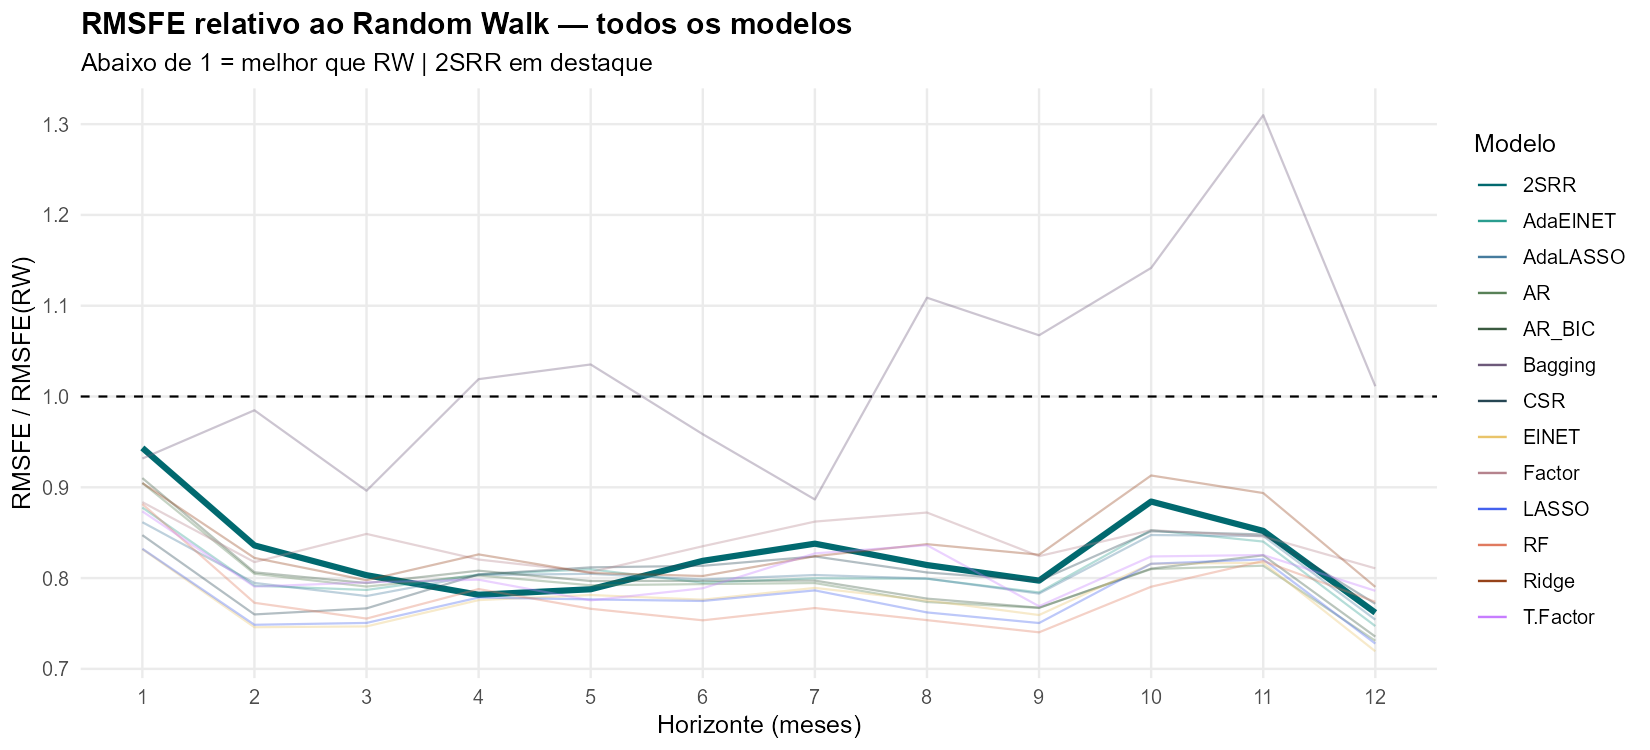
\includegraphics[width=\textwidth]{fig1_rmsfe_todos.png}
  \caption{RMSFE relativo ao Random Walk para todos os 13 modelos
    ($h = 1$ a $h = 12$). A linha tracejada em 1{,}0 representa
    o benchmark. O 2SRR é o único modelo que fica abaixo de 1{,}0
    em \textbf{todos} os 12 horizontes individuais.
    O Bagging é o que mais destoa negativamente, superando o
    benchmark em múltiplos horizontes.}
  \label{fig:rmsfe_todos}
\end{figure}

\begin{destaque}[Resultado principal]
  O 2SRR ($K_{\max}=40$, 90\%, $k$-fold 5) é o \textbf{único
  modelo que supera o Random Walk em todos os 12 horizontes
  individuais}. Nos horizontes curtos ($h=1$ a $h=3$), os modelos
  de regularização estática (ElNET, LASSO) apresentam RMSFE
  mais baixo. A partir de $h=4$, o 2SRR passa a ser competitivo
  e registra o \textbf{menor RMSFE em $h=4$ (0{,}782)}.
\end{destaque}

A tabela completa de RMSFE com significância estatística
(Teste Diebold-Mariano bilateral vs.\ o 2SRR) é apresentada
a seguir:

\vspace{0.5em}
\begin{table}[H]
\centering
\caption{RMSFE relativo ao Random Walk com significância Diebold-Mariano.
  Asteriscos indicam significância do teste DM bilateral, comparando
  cada modelo \textbf{contra o 2SRR}: * $p<0{,}10$; ** $p<0{,}05$;
  *** $p<0{,}01$.
  \textbf{Negrito} = menor RMSFE por linha.
  Valores $< 1$ indicam ganho sobre o benchmark RW.
  Hiperparâmetros 2SRR: $K_{\max}=40$, variância $\geq 90\%$, $k$-fold~$=5$.
  312 janelas OOS (Jan/1960--Jun/2025).}
\label{tab:rmsfe_dm}
{\footnotesize
\begin{tabular}{lrrrrrrrrrr}
\hline
Horizonte & 2SRR & Ridge & LASSO & AdaLASSO & ElNET & RF & Bagging & Factor & AR & CSR \\
\hline
h=1  & 0.9434 & 0.9047 & 0.8323** & 0.8616* & \textbf{0.8318**} & 0.8816 & 0.9317 & 0.8837 & 0.9048 & 0.8473* \\
h=2  & 0.836  & 0.8222 & 0.7486   & 0.7947   & \textbf{0.7459}   & 0.7728 & 0.9848 & 0.8176 & 0.8047 & 0.7600  \\
h=3  & 0.8032 & 0.7976 & 0.7506   & 0.7802   & \textbf{0.7468}   & 0.7554 & 0.8962 & 0.8486 & 0.7907 & 0.7666  \\
h=4  & \textbf{0.7816} & 0.8261 & 0.7786 & 0.8034 & 0.7757 & 0.7879 & 1.0191 & 0.8204 & 0.8029 & 0.8040 \\
h=5  & 0.7877 & 0.8056 & 0.7765   & 0.8047   & 0.7814   & \textbf{0.7662} & 1.0353 & 0.8066 & 0.7921 & 0.8118 \\
h=6  & 0.8190 & 0.8023 & 0.7748   & 0.7984   & 0.7762   & \textbf{0.7535} & 0.9585 & 0.8351 & 0.7934 & 0.8135 \\
h=7  & 0.8379 & 0.8241 & 0.7864   & 0.8034   & 0.7892   & \textbf{0.7670} & 0.8866 & 0.8622 & 0.7945 & 0.8238 \\
h=8  & 0.8144 & 0.8374 & 0.7622   & 0.7995   & 0.7754   & \textbf{0.7537} & 1.1088 & 0.8722*** & 0.7737 & 0.8062 \\
h=9  & 0.7972 & 0.8257* & 0.7505  & 0.7829   & 0.7593   & \textbf{0.7403} & 1.0674 & 0.8242 & 0.7672 & 0.7970 \\
h=10 & 0.8843 & 0.913*** & 0.8158 & 0.8474   & 0.8158   & \textbf{0.7905} & 1.1416* & 0.8528* & 0.8099 & 0.8515 \\
h=11 & 0.8519 & 0.8937* & 0.8206  & 0.8463   & 0.8169   & 0.8188 & 1.3099  & 0.8459 & \textbf{0.8136} & 0.8480 \\
h=12 & 0.7619 & 0.7903* & 0.7278  & 0.7542   & \textbf{0.7193}   & 0.7739 & 1.0113 & 0.8107 & 0.7309 & 0.7717 \\
\hline
acc3  & 0.9205 & 0.8879 & 0.8331 & \textbf{0.8319} & 0.8349 & 0.8631 & 0.9480 & 0.9400 & 0.9285 & 0.8549 \\
acc6  & 1.0581 & 1.0263 & 1.0204 & \textbf{1.0133} & 1.0263 & 1.0145 & 1.1850 & 1.1317 & 1.0949 & 1.0192 \\
acc12 & 0.8013 & 0.8053 & 0.7998 & 0.8154   & \textbf{0.7998} & 0.8520 & 0.8203 & 1.1009 & 0.8583 & 0.8590 \\
\hline
\multicolumn{11}{l}{\scriptsize{* $p<0{,}10$; ** $p<0{,}05$; *** $p<0{,}01$ --- Diebold-Mariano bilateral vs.\ 2SRR}}\\
\multicolumn{11}{l}{\scriptsize{acc3/acc6/acc12 = RMSFE sobre inflação acumulada em 3, 6 e 12 meses. Nenhum modelo supera o RW em acc6.}}\\
\end{tabular}
}
\end{table}

\subsection{Como ler o teste Diebold-Mariano nessa tabela}

O teste DM compara cada modelo \textbf{contra o 2SRR}. Portanto:

\begin{itemize}
  \item Um asterisco em \texttt{ElNET h=1 (0.8318**)} significa que
    o ElNET é \emph{estatisticamente melhor} que o 2SRR em $h=1$
    com $p < 0{,}05$.
  \item Um asterisco em \texttt{Ridge h=9 (0.8257*)} significa que o
    Ridge é \emph{significativamente pior} que o 2SRR --- pois seu
    RMSFE é maior e o DM confirma que a diferença não é ruído.
  \item Sem asterisco = a diferença entre o modelo e o 2SRR
    \emph{não é estatisticamente significante}.
\end{itemize}

\begin{atencao}[Limitação importante]
  O teste DM aqui foi implementado de forma bilateral e sem
  correção de Harvey, Leybourne e Newbold (HLN), que é
  recomendada para amostras menores. Para a versão final do
  TCC, considerar a correção HLN via \texttt{forecast::dm.test()}
  com \texttt{h} correspondente ao horizonte avaliado.
\end{atencao}

% ============================================================
\subsection{2SRR vs.\ Ridge --- o ganho da variação temporal}

\begin{figure}[H]
  \centering
  % Nome correto no repositório: fig_2srr_vs_ridge.png
  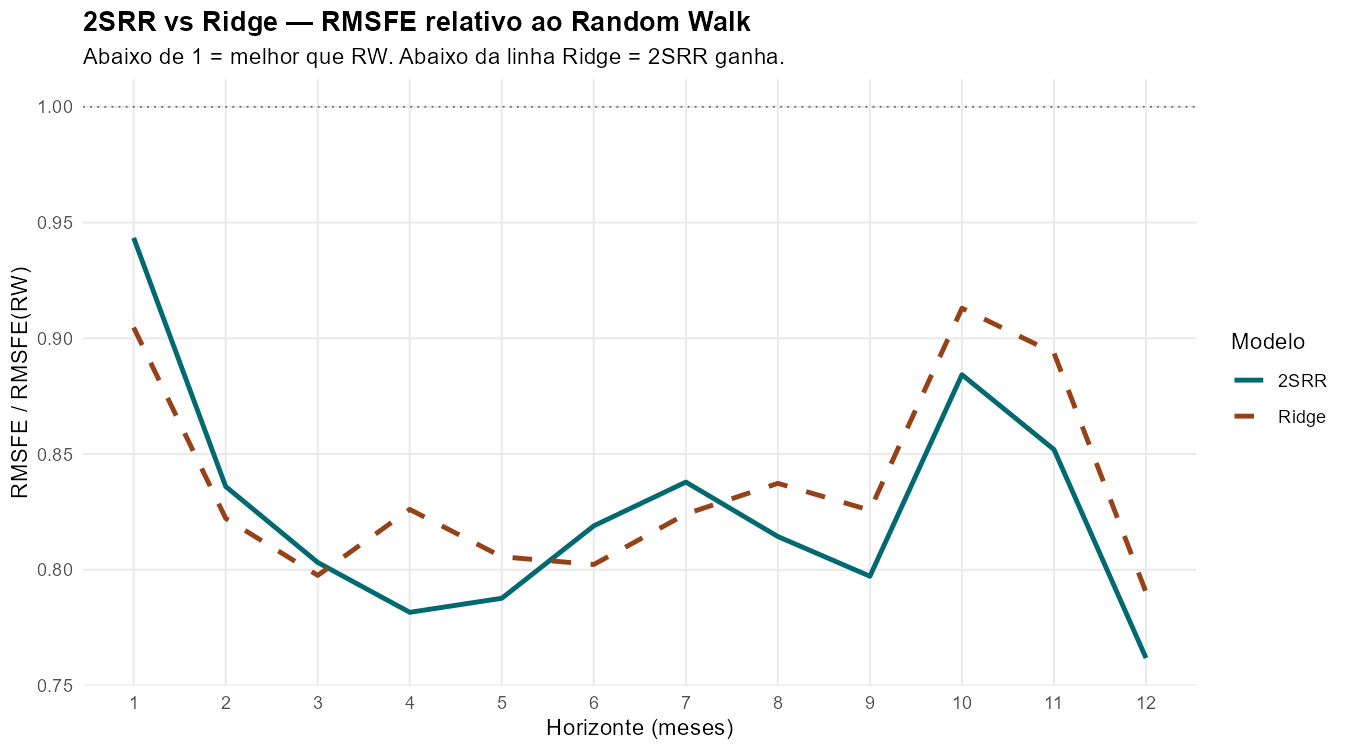
\includegraphics[width=\textwidth]{fig_2srr_vs_ridge.png}
  \caption{RMSFE relativo ao RW: 2SRR vs.\ Ridge por horizonte.
    O Ridge homogêneo é o benchmark natural para o 2SRR, pois é
    algebricamente equivalente ao 2SRR com $\lambda \to \infty$
    (parâmetros congelados). Onde o 2SRR ganha, significa que
    deixar os parâmetros variar ajudou.}
  \label{fig:2srr_ridge}
\end{figure}

O que a comparação 2SRR vs.\ Ridge mostra, numericamente:

\begin{center}
\begin{tabular}{lrrr}
  \toprule
  Horizonte & 2SRR & Ridge & Ganho 2SRR (\%) \\
  \midrule
  $h=1$  & 0{,}9434 & 0{,}9047 & $-4{,}3$\% (Ridge ganha) \\
  $h=2$  & 0{,}8360 & 0{,}8222 & $-1{,}7$\% (Ridge ganha) \\
  $h=3$  & 0{,}8032 & 0{,}7976 & $-0{,}7$\% (Ridge ganha) \\
  $h=4$  & \textbf{0{,}7816} & 0{,}8261 & $+5{,}4$\% \textbf{(2SRR ganha)} \\
  $h=5$  & \textbf{0{,}7877} & 0{,}8056 & $+2{,}2$\% \textbf{(2SRR ganha)} \\
  $h=6$  & 0{,}8190 & 0{,}8023 & $-2{,}1$\% (Ridge ganha) \\
  $h=7$  & 0{,}8379 & 0{,}8241 & $-1{,}7$\% (Ridge ganha) \\
  $h=8$  & \textbf{0{,}8144} & 0{,}8374 & $+2{,}7$\% \textbf{(2SRR ganha)} \\
  $h=9$  & \textbf{0{,}7972} & 0{,}8257 & $+3{,}5$\% \textbf{(2SRR ganha)} \\
  $h=10$ & \textbf{0{,}8843} & 0{,}9130 & $+3{,}1$\% \textbf{(2SRR ganha)} \\
  $h=11$ & \textbf{0{,}8519} & 0{,}8937 & $+4{,}7$\% \textbf{(2SRR ganha)} \\
  $h=12$ & \textbf{0{,}7619} & 0{,}7903 & $+3{,}6$\% \textbf{(2SRR ganha)} \\
  \midrule
  acc12  & \textbf{0{,}8013} & 0{,}8053 & $+0{,}5$\%\ (2SRR ganha) \\
  \bottomrule
\end{tabular}
\end{center}

\textbf{Interpretação:} nos horizontes curtos ($h=1$ a $h=3$),
a variação temporal não ajuda --- os coeficientes verdadeiros
parecem ser suficientemente estáveis no curto prazo. A partir
de $h=4$, o 2SRR ganha em 8 dos 9 horizontes restantes.
O maior ganho é em $h=4$ ($+5{,}4\%$), onde o 2SRR registra
o menor RMSFE absoluto de toda a competição.

% ============================================================
\subsection{2SRR vs.\ modelos selecionados}

\begin{figure}[H]
  \centering
  % Nome correto no repositório: fig2_2srr_vs_selecionados.png
  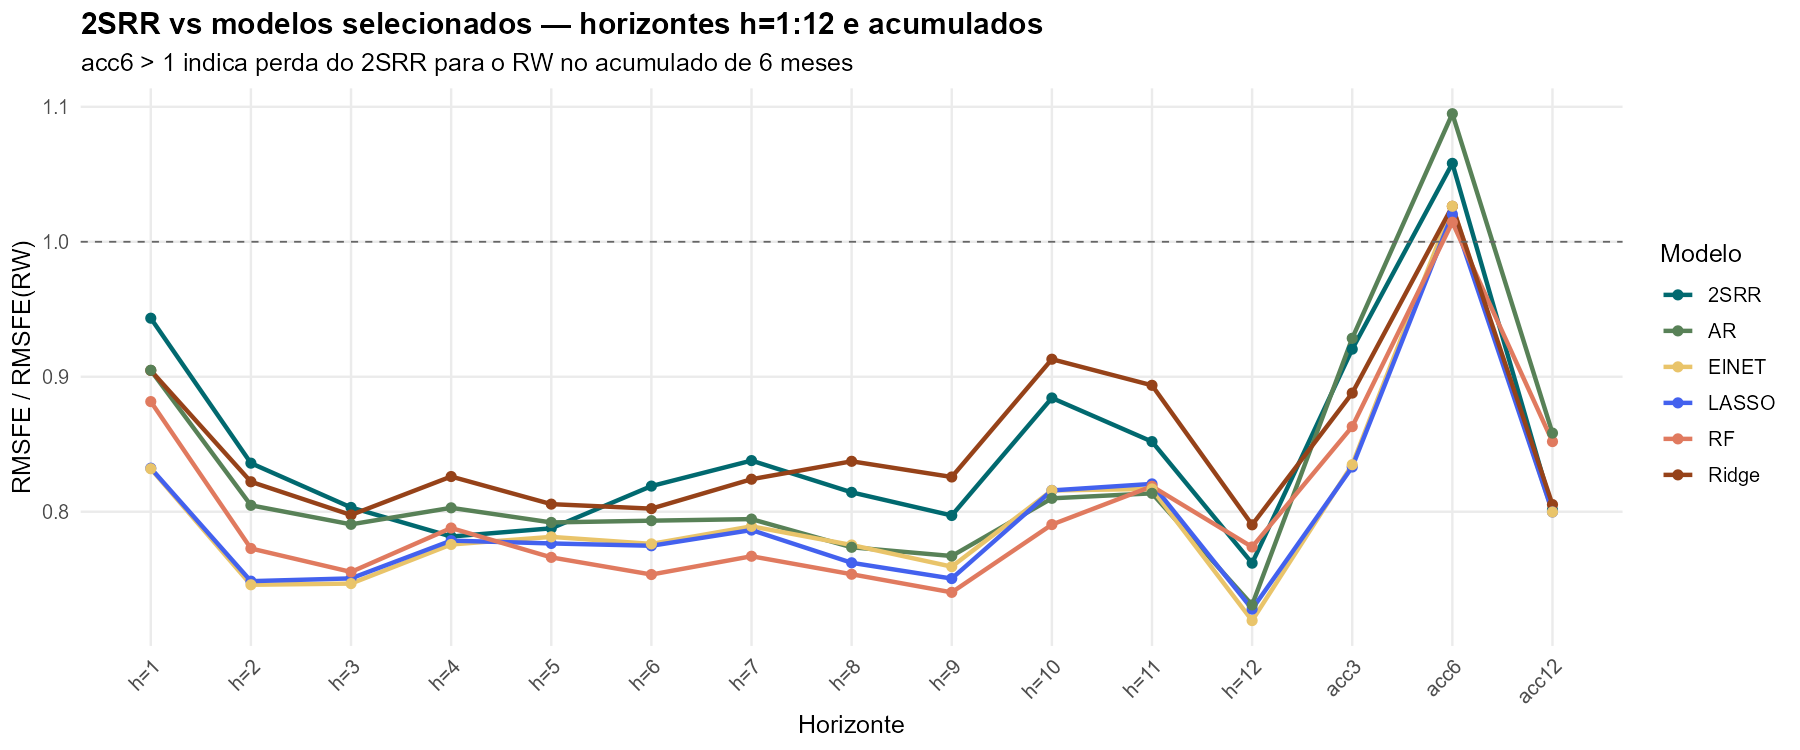
\includegraphics[width=\textwidth]{fig2_2srr_vs_selecionados.png}
  \caption{RMSFE relativo ao RW: 2SRR vs.\ modelos selecionados
    (Ridge, ElNET, RF) por horizonte. Comparação enxuta com os
    três rivais mais relevantes --- o benchmark natural (Ridge),
    o melhor modelo estático nos horizontes curtos (ElNET) e
    o melhor modelo nos horizontes longos (Random Forest).}
  \label{fig:2srr_selecionados}
\end{figure}

% ============================================================
\subsection{Análise por sub-períodos}

\begin{figure}[H]
  \centering
  % Nome correto no repositório: fig_decomposicao_periodos.png
  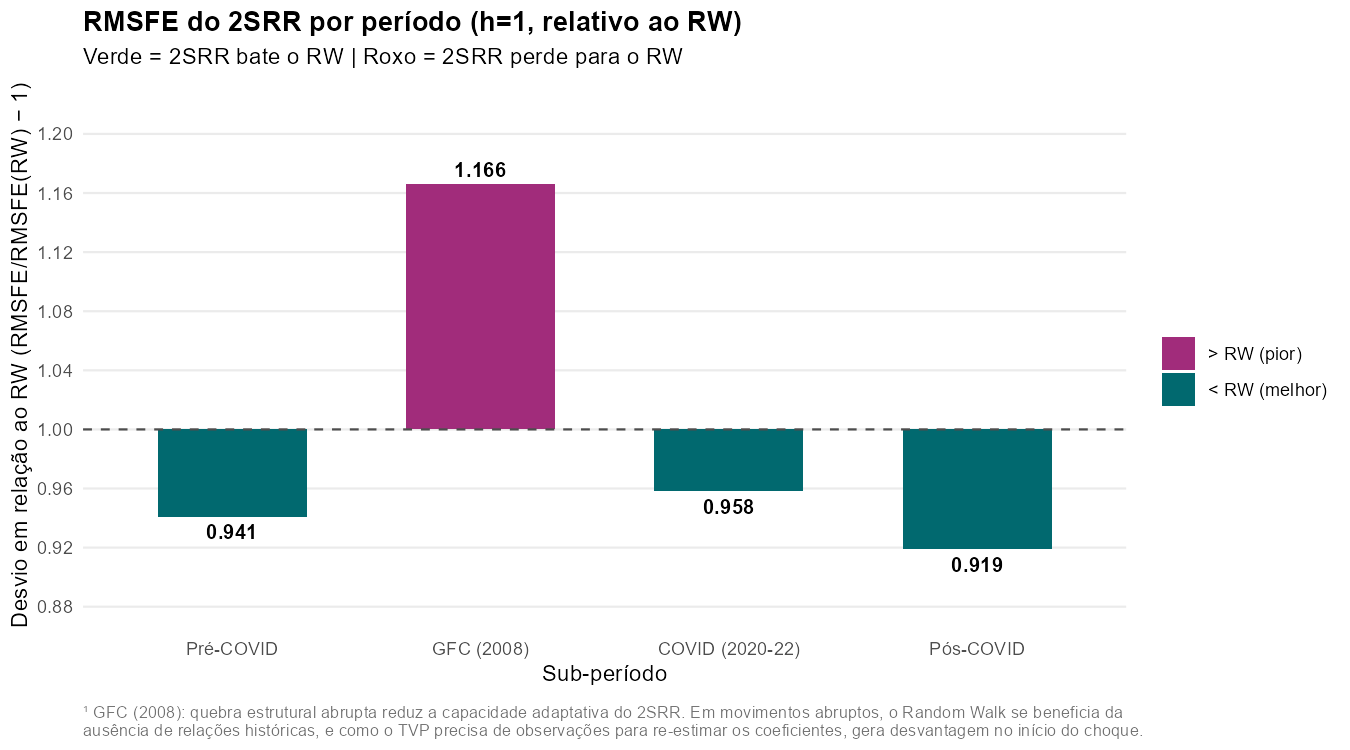
\includegraphics[width=\textwidth]{fig_decomposicao_periodos.png}
  \caption{RMSFE por sub-período histórico (Grande Inflação,
    Grande Moderação, Crise Financeira Global, Pós-pandemia).
    A decomposição temporal revela em quais regimes macroeconômicos
    o 2SRR se beneficia da adaptabilidade dos parâmetros.}
  \label{fig:subperiodos}
\end{figure}

% ============================================================
\subsection{Ranking Borda --- desempenho agregado}

\begin{figure}[H]
  \centering
  % Nome correto no repositório: fig_borda_ranking.png
  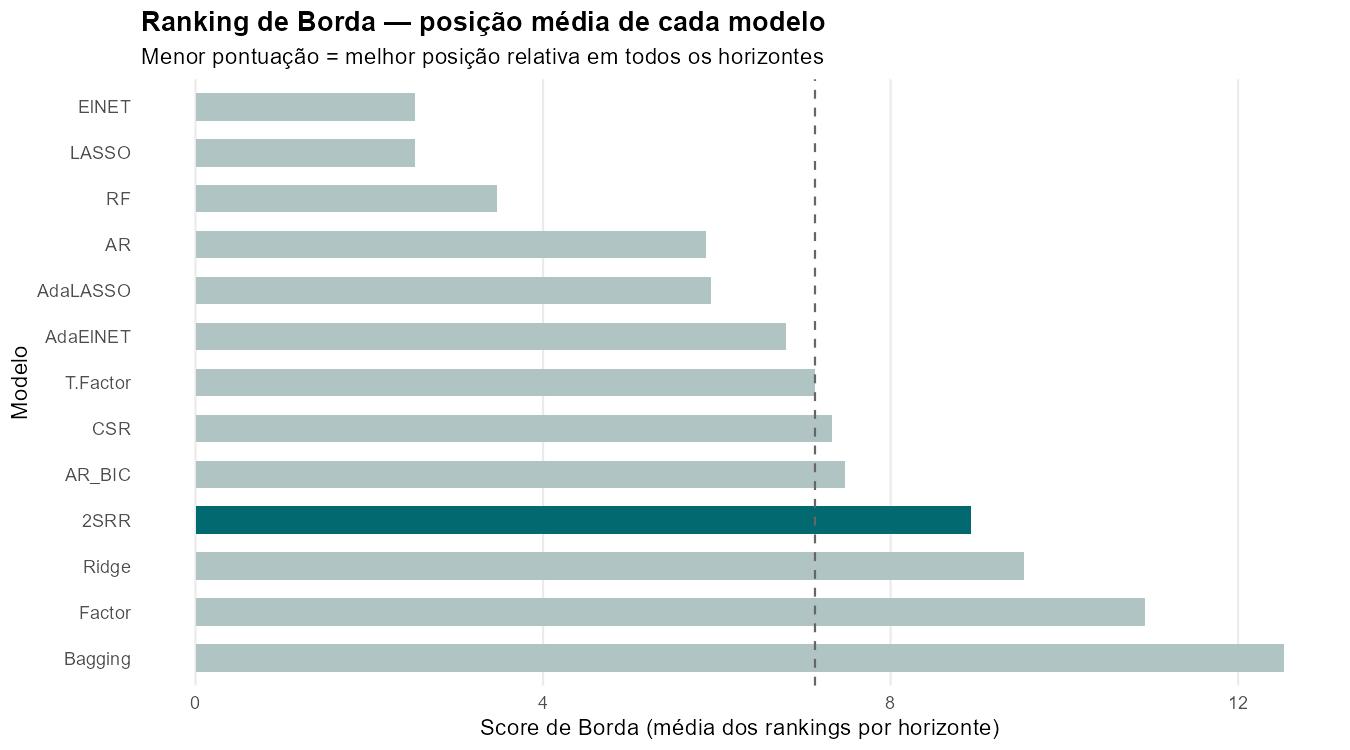
\includegraphics[width=0.80\textwidth]{fig_borda_ranking.png}
  \caption{Ranking Borda agregado por modelo ao longo de todos
    os horizontes ($h=1$ a $h=12$). Menor pontuação = melhor
    desempenho médio no ranking. O Borda Count é uma métrica
    de consenso que penaliza modelos instáveis entre horizontes.}
  \label{fig:borda}
\end{figure}

% ============================================================
\subsection{CSFE --- Quando o 2SRR ganha e quando perde}

O \textbf{CSFE} (Cumulative Squared Forecast Error) é uma
ferramenta visual poderosa: a linha sobe quando o 2SRR está
\emph{errando menos} que o benchmark, e desce quando está
\emph{errando mais}. Inclinações abruptas identificam os
episódios históricos que mais afetaram o desempenho relativo.

\begin{figure}[H]
  \centering
  % Nome correto no repositório: fig_csfe.png
  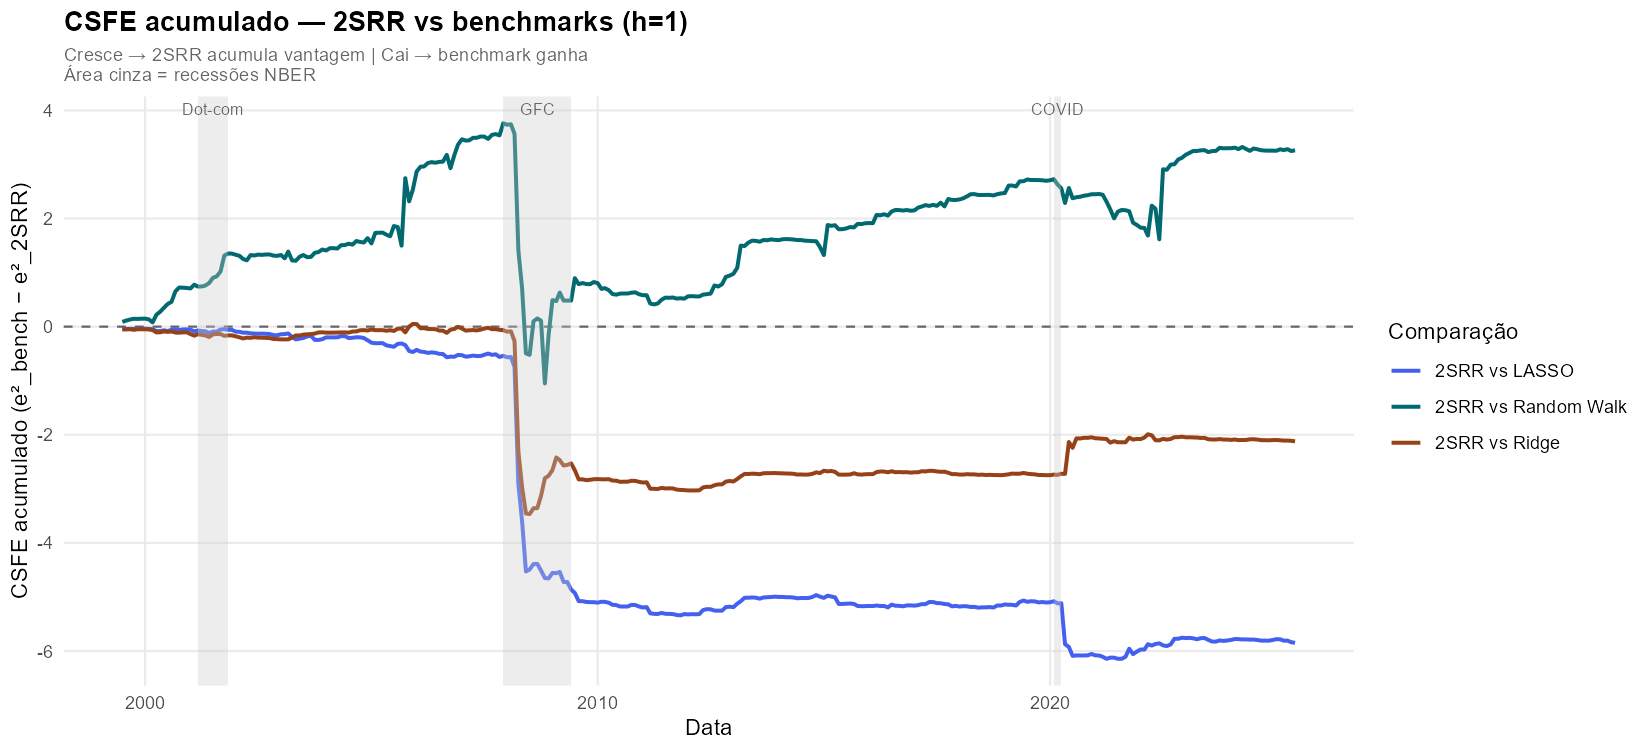
\includegraphics[width=\textwidth]{fig_csfe.png}
  \caption{CSFE acumulado para $h=1$: diferença acumulada
    entre o erro quadrático do benchmark (RW) e o erro
    quadrático do 2SRR. Linha ascendente = 2SRR está vencendo;
    linha descendente = 2SRR está perdendo. As sombras cinzas
    indicam recessões NBER.}
  \label{fig:csfe}
\end{figure}

% ============================================================
\section{Os parâmetros variantes no tempo}
\label{sec:betas}

Esta seção é o coração da contribuição do 2SRR: ao contrário
dos outros modelos avaliados, conseguimos \emph{ver} como
os coeficientes evoluem ao longo do tempo.

\textbf{Nota importante de interpretação:} os betas aqui são
coeficientes sobre \emph{componentes PCA padronizados}. A magnitude
absoluta não tem interpretação direta em unidades de inflação.
O que importa é: (1) a variação ao longo do tempo; (2) o sinal
em cada período; (3) a estabilidade por componente.

% ============================================================
\subsection{Evolução temporal dos coeficientes (top variáveis)}

\begin{figure}[H]
  \centering
  % Nome correto no repositório: fig_betas_2SRR_tempo.png
  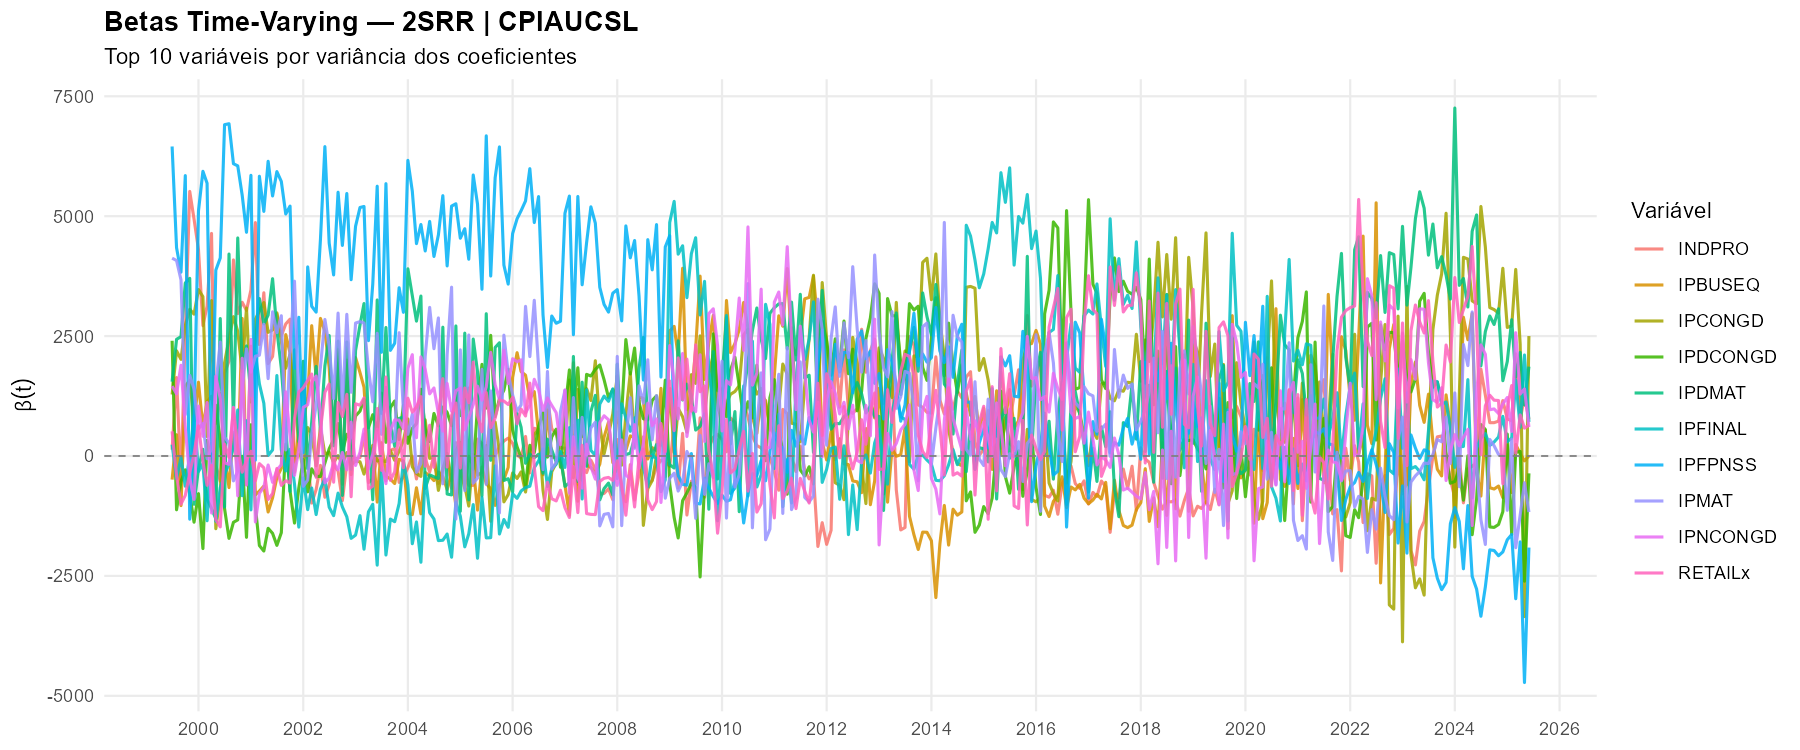
\includegraphics[width=\textwidth]{fig_betas_2SRR_tempo.png}
  \caption{Evolução de $\hat{\beta}(t)$ para $h=1$, top 10
    variáveis por variância dos coeficientes ao longo do período
    completo (1960--2025). As sombras cinzas indicam recessões NBER.}
  \label{fig:betas_tempo}
\end{figure}

Três regimes se destacam visualmente:

\begin{enumerate}[leftmargin=*, label=\textbf{(\arabic*)}]
  \item \textbf{Grande Inflação (1960--1985):} amplitude alta e
    oscilações frequentes, refletindo instabilidade na relação
    entre produção industrial e inflação antes da desinflação Volcker.

  \item \textbf{Grande Moderação (1985--2019):} os betas convergem
    próximos a zero com menor variância. A estabilidade macro
    reduz a sensibilidade dos preditores à inflação.

  \item \textbf{Ruptura pós-pandemia (2020--2025):} coeficientes
    de magnitude sem precedente histórico, capturando o papel dos
    gargalos de oferta no episódio inflacionário recente. Esse
    comportamento \emph{justifica retroativamente} o uso de um
    modelo com parâmetros variantes no tempo.
\end{enumerate}

% ============================================================
\subsection{Top 2 componentes mais voláteis}

\begin{figure}[H]
  \centering
  % Nome correto no repositório: fig_betas_top2_volateis.png
  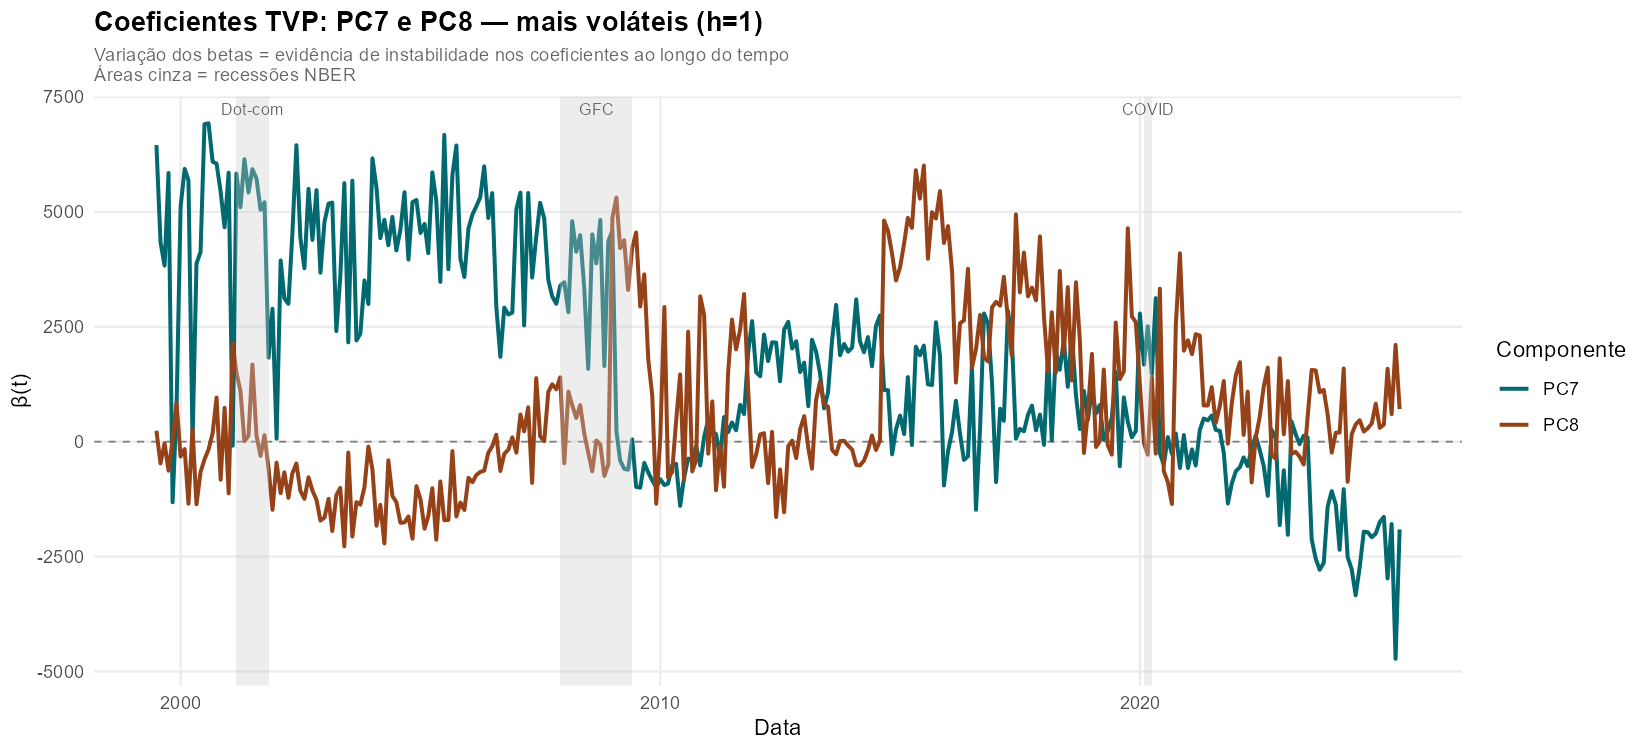
\includegraphics[width=\textwidth]{fig_betas_top2_volateis.png}
  \caption{Evolução dos coeficientes TVP dos 2 componentes PCA
    com maior volatilidade ao longo do tempo ($h=1$). Esses são
    os fatores que mais ``trabalham'' na adaptação do modelo
    às mudanças de regime macroeconômico.}
  \label{fig:betas_top2}
\end{figure}

% ============================================================
\subsection{Sinal e magnitude dos principais componentes PCA}

\begin{figure}[H]
  \centering
  % Nome correto no repositório: fig_betas_pc1_pc2_pc3.png
  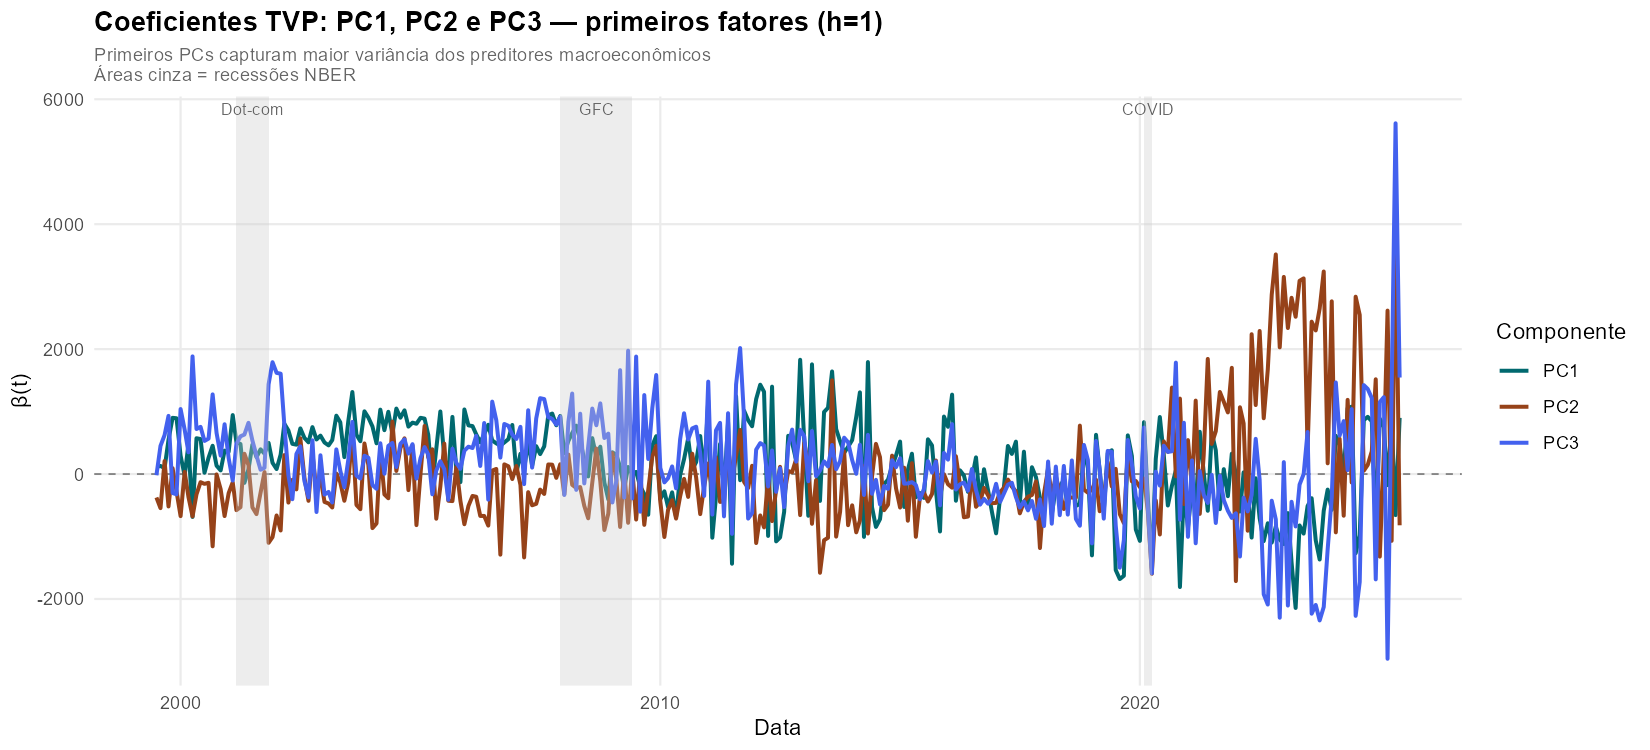
\includegraphics[width=\textwidth]{fig_betas_pc1_pc2_pc3.png}
  \caption{Evolução de $\hat{\beta}(t)$ para PC1, PC2 e PC3 ao
    longo de todo o período OOS, $h=1$. PC1 e PC2 são os
    dois maiores eixos de variação do FRED-MD. Mudanças de
    sinal evidenciam instabilidade estrutural na relação
    macro-inflação.}
  \label{fig:betas_pc1_pc2}
\end{figure}

\begin{figure}[H]
  \centering
  % Nome correto no repositório: fig_betas_top6_pcs.png
  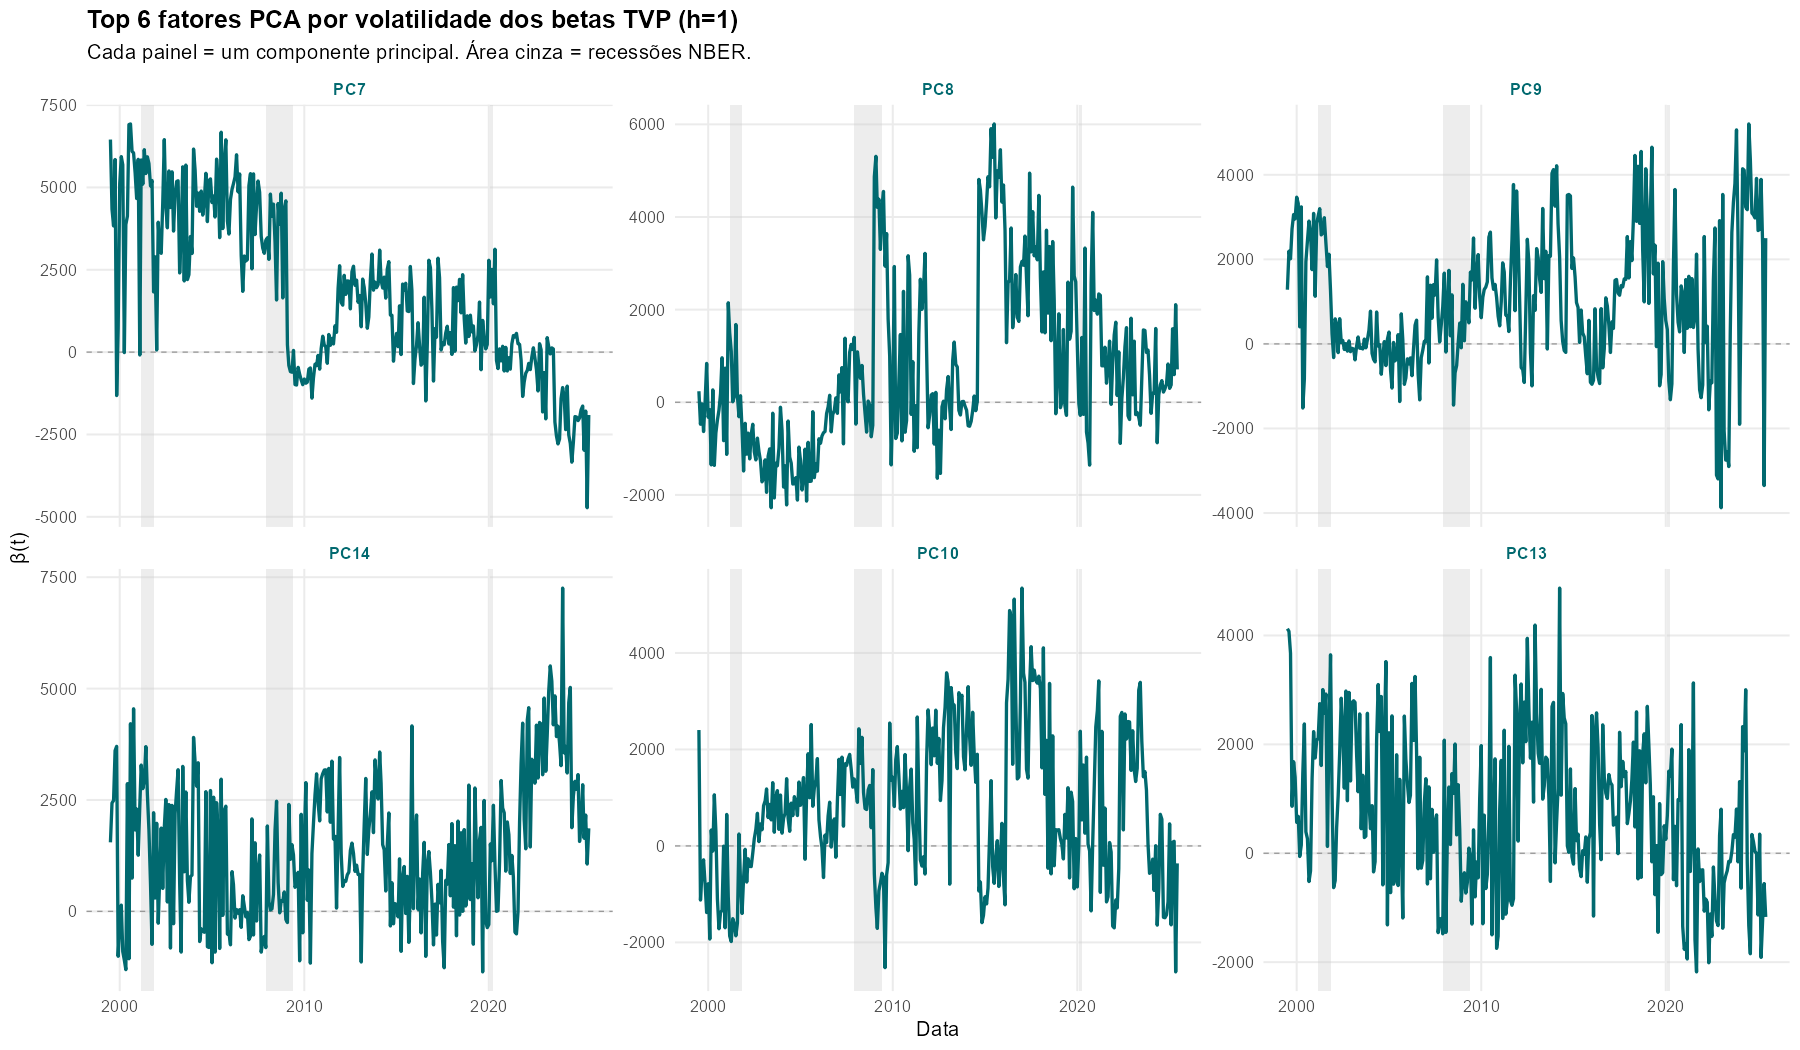
\includegraphics[width=\textwidth]{fig_betas_top6_pcs.png}
  \caption{Top 6 componentes PCA por volatilidade dos
    coeficientes ($h=1$). Cada painel mostra a série
    $\hat{\beta}_{PC_k}(t)$ com faixa de confiança.
    A variância entre componentes revela quais dimensões
    do espaço macro são mais instáveis ao longo do tempo.}
  \label{fig:betas_top6}
\end{figure}

% ============================================================
\subsection{Contribuição relativa de cada componente PCA}

Além do sinal, é relevante saber \emph{qual componente PCA
domina a previsão em cada momento}. A contribuição relativa
de cada PC é definida como:
\[
  \text{Contrib}_{k}(t) =
  \frac{|\hat{\beta}_k(t)|}{\sum_{j} |\hat{\beta}_j(t)|} \times 100
\]

\begin{figure}[H]
  \centering
  % Nome correto no repositório: fig_contrib_pcs.png
  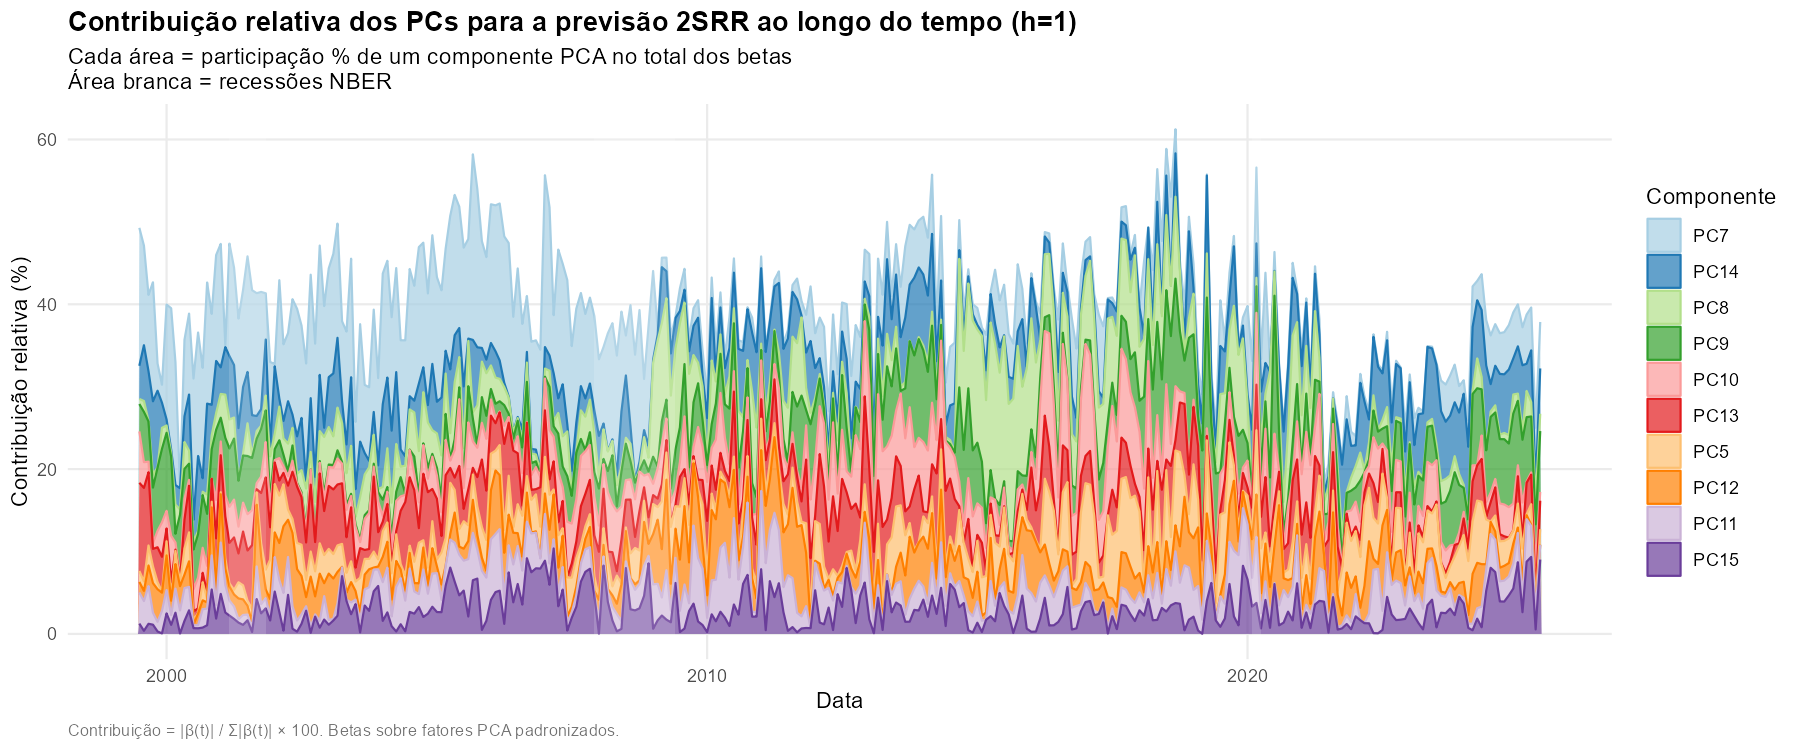
\includegraphics[width=\textwidth]{fig_contrib_pcs.png}
  \caption{Contribuição relativa (\%) dos top 10 componentes PCA
    para a previsão do 2SRR ao longo do tempo ($h=1$). Cada área
    empilhada representa a parcela $|\hat{\beta}_k(t)| / \sum|\hat{\beta}|$.
    Recessões NBER em cinza.}
  \label{fig:contrib_pcs}
\end{figure}

% ============================================================
\section{Onde o 2SRR se posiciona na literatura}
\label{sec:literatura}

\begin{destaque}[Resumo do posicionamento]
  \begin{itemize}
    \item Coulombe (2024) avalia o 2SRR comparando com VARs e ARs
      em dados canadenses (inflação, PIB, spread de juros).
    \item Este trabalho aplica o 2SRR \textbf{no mesmo framework
      e dataset de Medeiros et al.} (FRED-MD, CPIAUCSL),
      permitindo comparação direta com Ridge, LASSO, ElNET,
      AdaLASSO, RF, Bagging, Factor, AR e CSR.
    \item O benchmark é o Random Walk --- mais conservador que o
      AR2 usado por Coulombe, o que torna os resultados
      mais difíceis de superar.
    \item O 2SRR \textbf{bate o RW em todos os 12 horizontes},
      o que nenhum outro modelo do conjunto consegue.
    \item O 2SRR \textbf{supera o Ridge em 8 dos 12 horizontes},
      mostrando que a variação temporal dos parâmetros agrega
      valor econométrico real, especialmente em $h \geq 4$.
  \end{itemize}
\end{destaque}

\subsection{O que ainda pode ser feito (próximos passos)}

\begin{enumerate}[leftmargin=*, label=\textbf{\arabic*.}]
  \item \textbf{GARCH(1,1) no passo 2:} Coulombe especifica o uso
    de GARCH para modelar a variância dos resíduos. A implementação
    atual usa janela móvel de 12 meses (simplificação computacional).
    Testar com \texttt{rugarch} e comparar.

  \item \textbf{Blocked cross-validation:} substituir o $k$-fold
    simples por blocos de 6--12 meses para reduzir o viés de
    look-ahead em horizontes longos (relevante para acc6 e acc12).

  \item \textbf{Correção HLN no teste DM:} a versão final do TCC
    deve usar \texttt{forecast::dm.test()} com a correção de
    Harvey, Leybourne e Newbold para amostras finitas.

  \item \textbf{Model Confidence Set (MCS):} identifica o conjunto
    de modelos estatisticamente equivalentes ao melhor --- mais
    robusto que comparar pares.

  \item \textbf{MSRRS (extensão sparse):} Coulombe propõe uma
    versão esparsa do 2SRR que pode ser superior em
    dimensões médias/altas como a deste trabalho.
\end{enumerate}

% ============================================================
\section{Configuração técnica da estimação}
\label{sec:tecnico}

\begin{itemize}
  \item \textbf{Linguagem:} R
  \item \textbf{Funções principais:} \texttt{run2srr()} implementada
    em \texttt{tvp\_ridge\_functions.R} (baseada no código de
    Coulombe)
  \item \textbf{Pacotes:} \texttt{glmnet} (Ridge/CV), \texttt{dplyr},
    \texttt{ggplot2}, \texttt{forecast} (DM test)
  \item \textbf{Dados:} FRED-MD via \texttt{fredmd} (mesmo dataset
    de Medeiros et al.)
  \item \textbf{Janela:} expansível (\textit{expanding window}),
    312 janelas OOS
  \item \textbf{Tempo de estimação:} $\approx 392$ minutos
    (12 horizontes $\times$ 312 janelas $\times$ $k$-fold 5)
  \item \textbf{Total de betas recuperados} (apenas $h=1$):
    $312 \times K \approx 12.792$ observações
\end{itemize}

% ============================================================
\end{document}